
	\section{相对运动}
	\subsection{使用前提}
	参考系$K$相对于参考系$K'$作\textbf{平动}。$K'$系的坐标原点$O'$相当于$K$系可作任意的直线或曲线运动，但它们的坐标轴的方向总是保持不变。

	\begin{figure}[h]
		\centering
		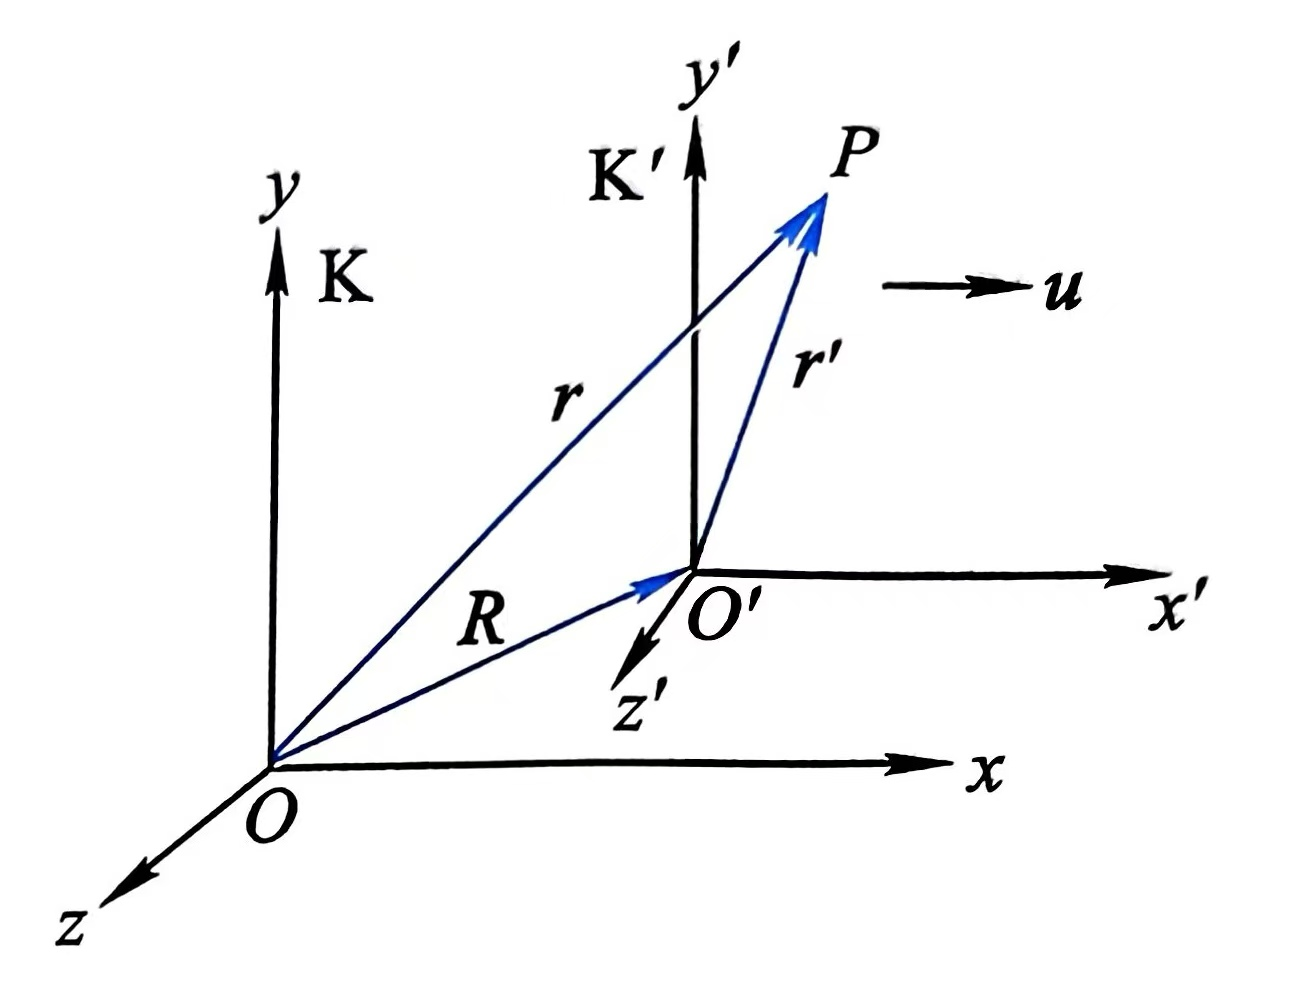
\includegraphics[width=0.5\textwidth]{images/revelate.jpg}
		\caption{相对运动关系图解}
	\end{figure}
	
	\subsection{重要公式}
	\subsubsection{位矢关系}
	
	$\vec{r}$：质点$P$在$K$系中的位矢。
	
	$\vec{r'}$：质点$P$在$K'$系中的位矢。
	
	$\vec{R}$：$K'$系原点$O'$对$K$系原点$O$的位矢。
		$$\vec{r}=\vec{r'}+\vec{R}$$
	
	\subsubsection{速度关系}
	
	绝对速度$\vec{v}$：质点相对于静止参考系$K$的速度。
	
	相对速度$\vec{v'}$：质点相对于运动参考系$K'$的速度。
	
	牵连速度$\vec{u}$：两参考系之间的相对速度。
		$$\vec{v}=\vec{v'}+\vec{u}$$
	
	\subsubsection{加速度关系}
	
	$\vec{a}$：质点相对于静止参考系$K$的加速度。
	
	$\vec{a'}$：质点相对于运动参考系$K'$的加速度。
	
	$\vec{a_0}$：两参考系之间的相对加速度。
	
		$$\vec{a}=\vec{a'}+\vec{a_0}$$
	
	特别地，若$\vec{a_0}=0$，则$\vec{a}=\vec{a'}$。表明质点在两个相对作匀速直线运动的参考系中的加速度是相等的。质点的加速度相对于作匀速直线运动的各个参考系是个绝对量。
	
